\documentclass{article}
\usepackage{tikz}

\begin{document}

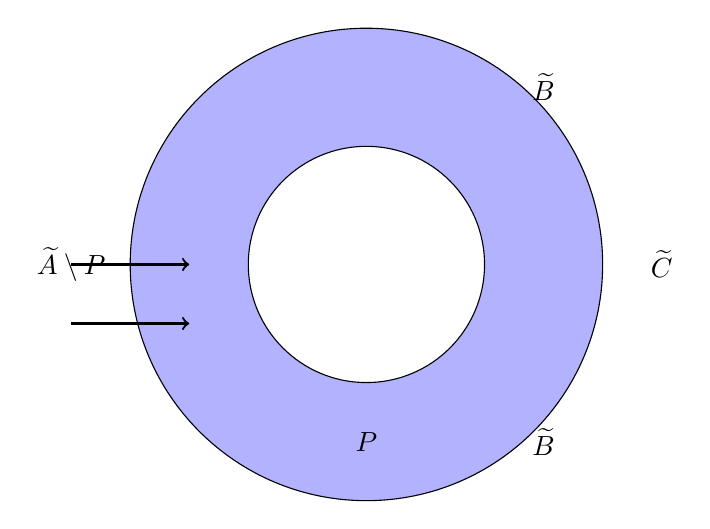
\begin{tikzpicture}[scale=1.5]
    % Draw the outer circle
    \draw[fill=blue!30] (0,0) circle (2cm);
    
    % Draw the inner circle
    \draw[fill=white] (0,0) circle (1cm);
    
    % Define the labels
    \node at (-2.5, 0) {$\widetilde{A} \setminus P$};
    \node at (0, -1.5) {$P$};
    \node at (1.5, 1.5) {$\widetilde{B}$};
    \node at (1.5, -1.5) {$\widetilde{B}$};
    \node at (2.5, 0) {$\widetilde{C}$};
    
    % Draw the arrows
    \draw[->, thick] (-2.5, 0) -- (-1.5, 0);
    \draw[->, thick] (-2.5, -0.5) -- (-1.5, -0.5);
\end{tikzpicture}

\end{document}